\section{Diskussion}
\label{sec:Diskussion}

In der Auswertung dieses Versuches konnten also anhand der Evakuierungs- und Leckratenmessungen unterschiedliche Ergebnisse für das Saugvermögen in unterschiedlichen Druckbereichen für beide Pumpentypen bestimmt werden.  Als Endergebnis werden diese in \autoref{fig:plotts} und \autoref{fig:plotds} zusammengefasst und mit dem vom Hersteller angegebenen Theoriewert verglichen.

\begin{figure}[H]
    \centering
    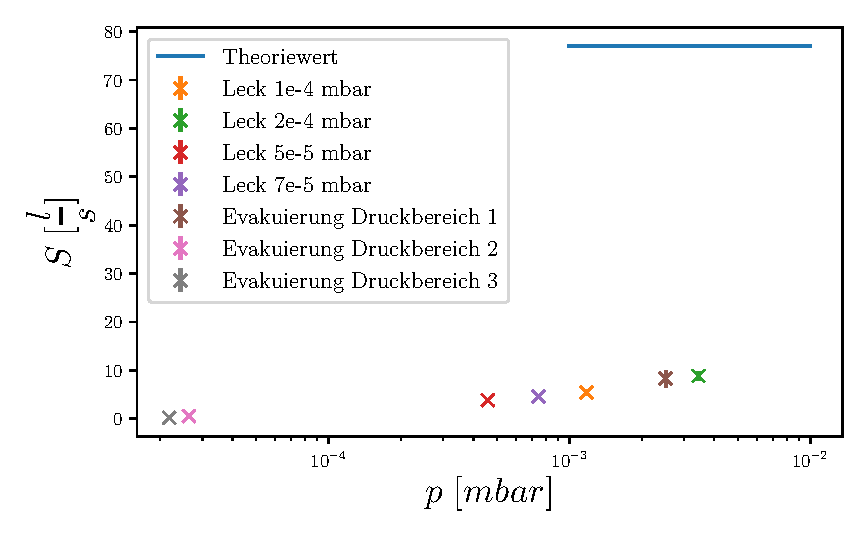
\includegraphics{build/plots/saug_turbo.pdf}
    \caption{Berechnetes Saugvermögen in Abhängigkeit des Drucks und Vergleich mit dem Theoriewert für die Turbopumpe}
    \label{fig:plotts}
  \end{figure}
\noindent
An \autoref{fig:plotts} ist zu sehen, dass die Ergebnisse für das Saugvermögen für die Turbopumpe stark von dem vom Hersteller angegebenen Theroriewert abweichen. Die hohe Abweichung ist teilweise dadurch zu erklären, dass die Messwerte in gewisser Entfernung von der Turbomolekularpumpe aufgenommen wurden, sodass der Leitwert die Saugleistung verringert. Dazu wurden allgemein die vom Hersteller angegebenen Idealbedingungen für die Nutzung der Pumpe nicht erreicht.


\begin{figure}[H]
    \centering
    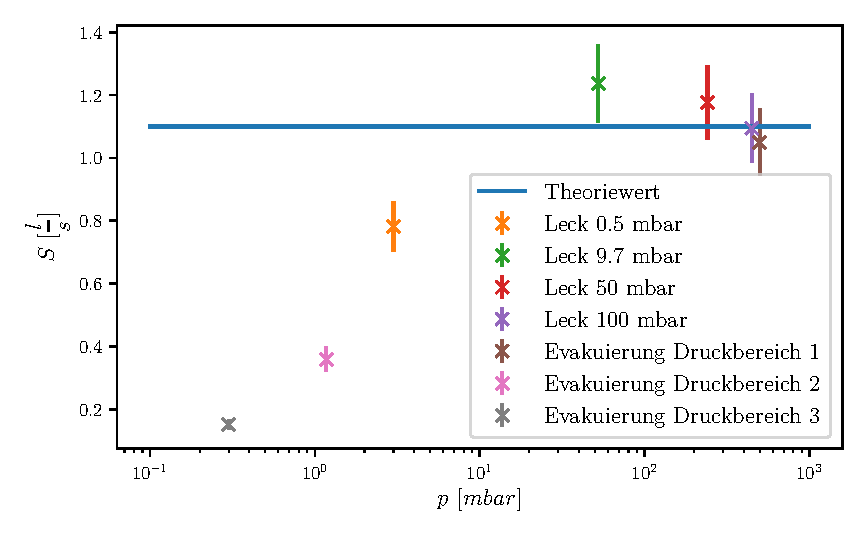
\includegraphics{build/plots/saug_dreh.pdf}
    \caption{Berechnetes Saugvermögen in Abhängigkeit des Drucks und Vergleich mit dem Theoriewert für die Drehschieberpumpe}
    \label{fig:plotds}
  \end{figure}
  \noindent
  Es ist zu sehen, dass das berechnete Saugvermögen für die Leckratenmessung bei $p_g = \SI{100}{\milli\bar}$ mit$(1.09 \pm 0.11) l/s$ sehr nah am Theoriewert von $1.1\ l/s$ liegt. Andererseits ist eine große Abweichung bei den niedrigeren Druckwerten bei der Evakuierungsmessung zu erkennen. Insgesamt ist zu sehen, dass die Ergebnisse bei höheren Druckwerten deutlich näher am Theoriewert liegen. \\
  Da Effekte wie die Verringerung der Saugleistung durch den Leitwert oder durch andere Einflüsse wie Desorption im Hochvakuum-Bereich eine größere Rolle spielen, kann es erklärt werden, dass die Ergebnisse für die Drehschieberpumpe generell näher an den Theoriewerten liegen als die Ergebnisse für die Turbomolekularpumpe.   